%*****************************************
\chapter{Stand der Forschung}\label{ch:relatedWork}
%*****************************************

\section{Die Ontologie: SNIK}

Das semantische Netz des Informationsmanagements im Krankenhaus (\ac{snik}) ist eine die Domäne des Informationsmanagements im Krankenhaus betreffende Ontologie.
Sie behandelt
\todo{SNIK}
\todo{Textbücher referenzieren}
\begin{sidewaysfigure}[htbp!]
\centering
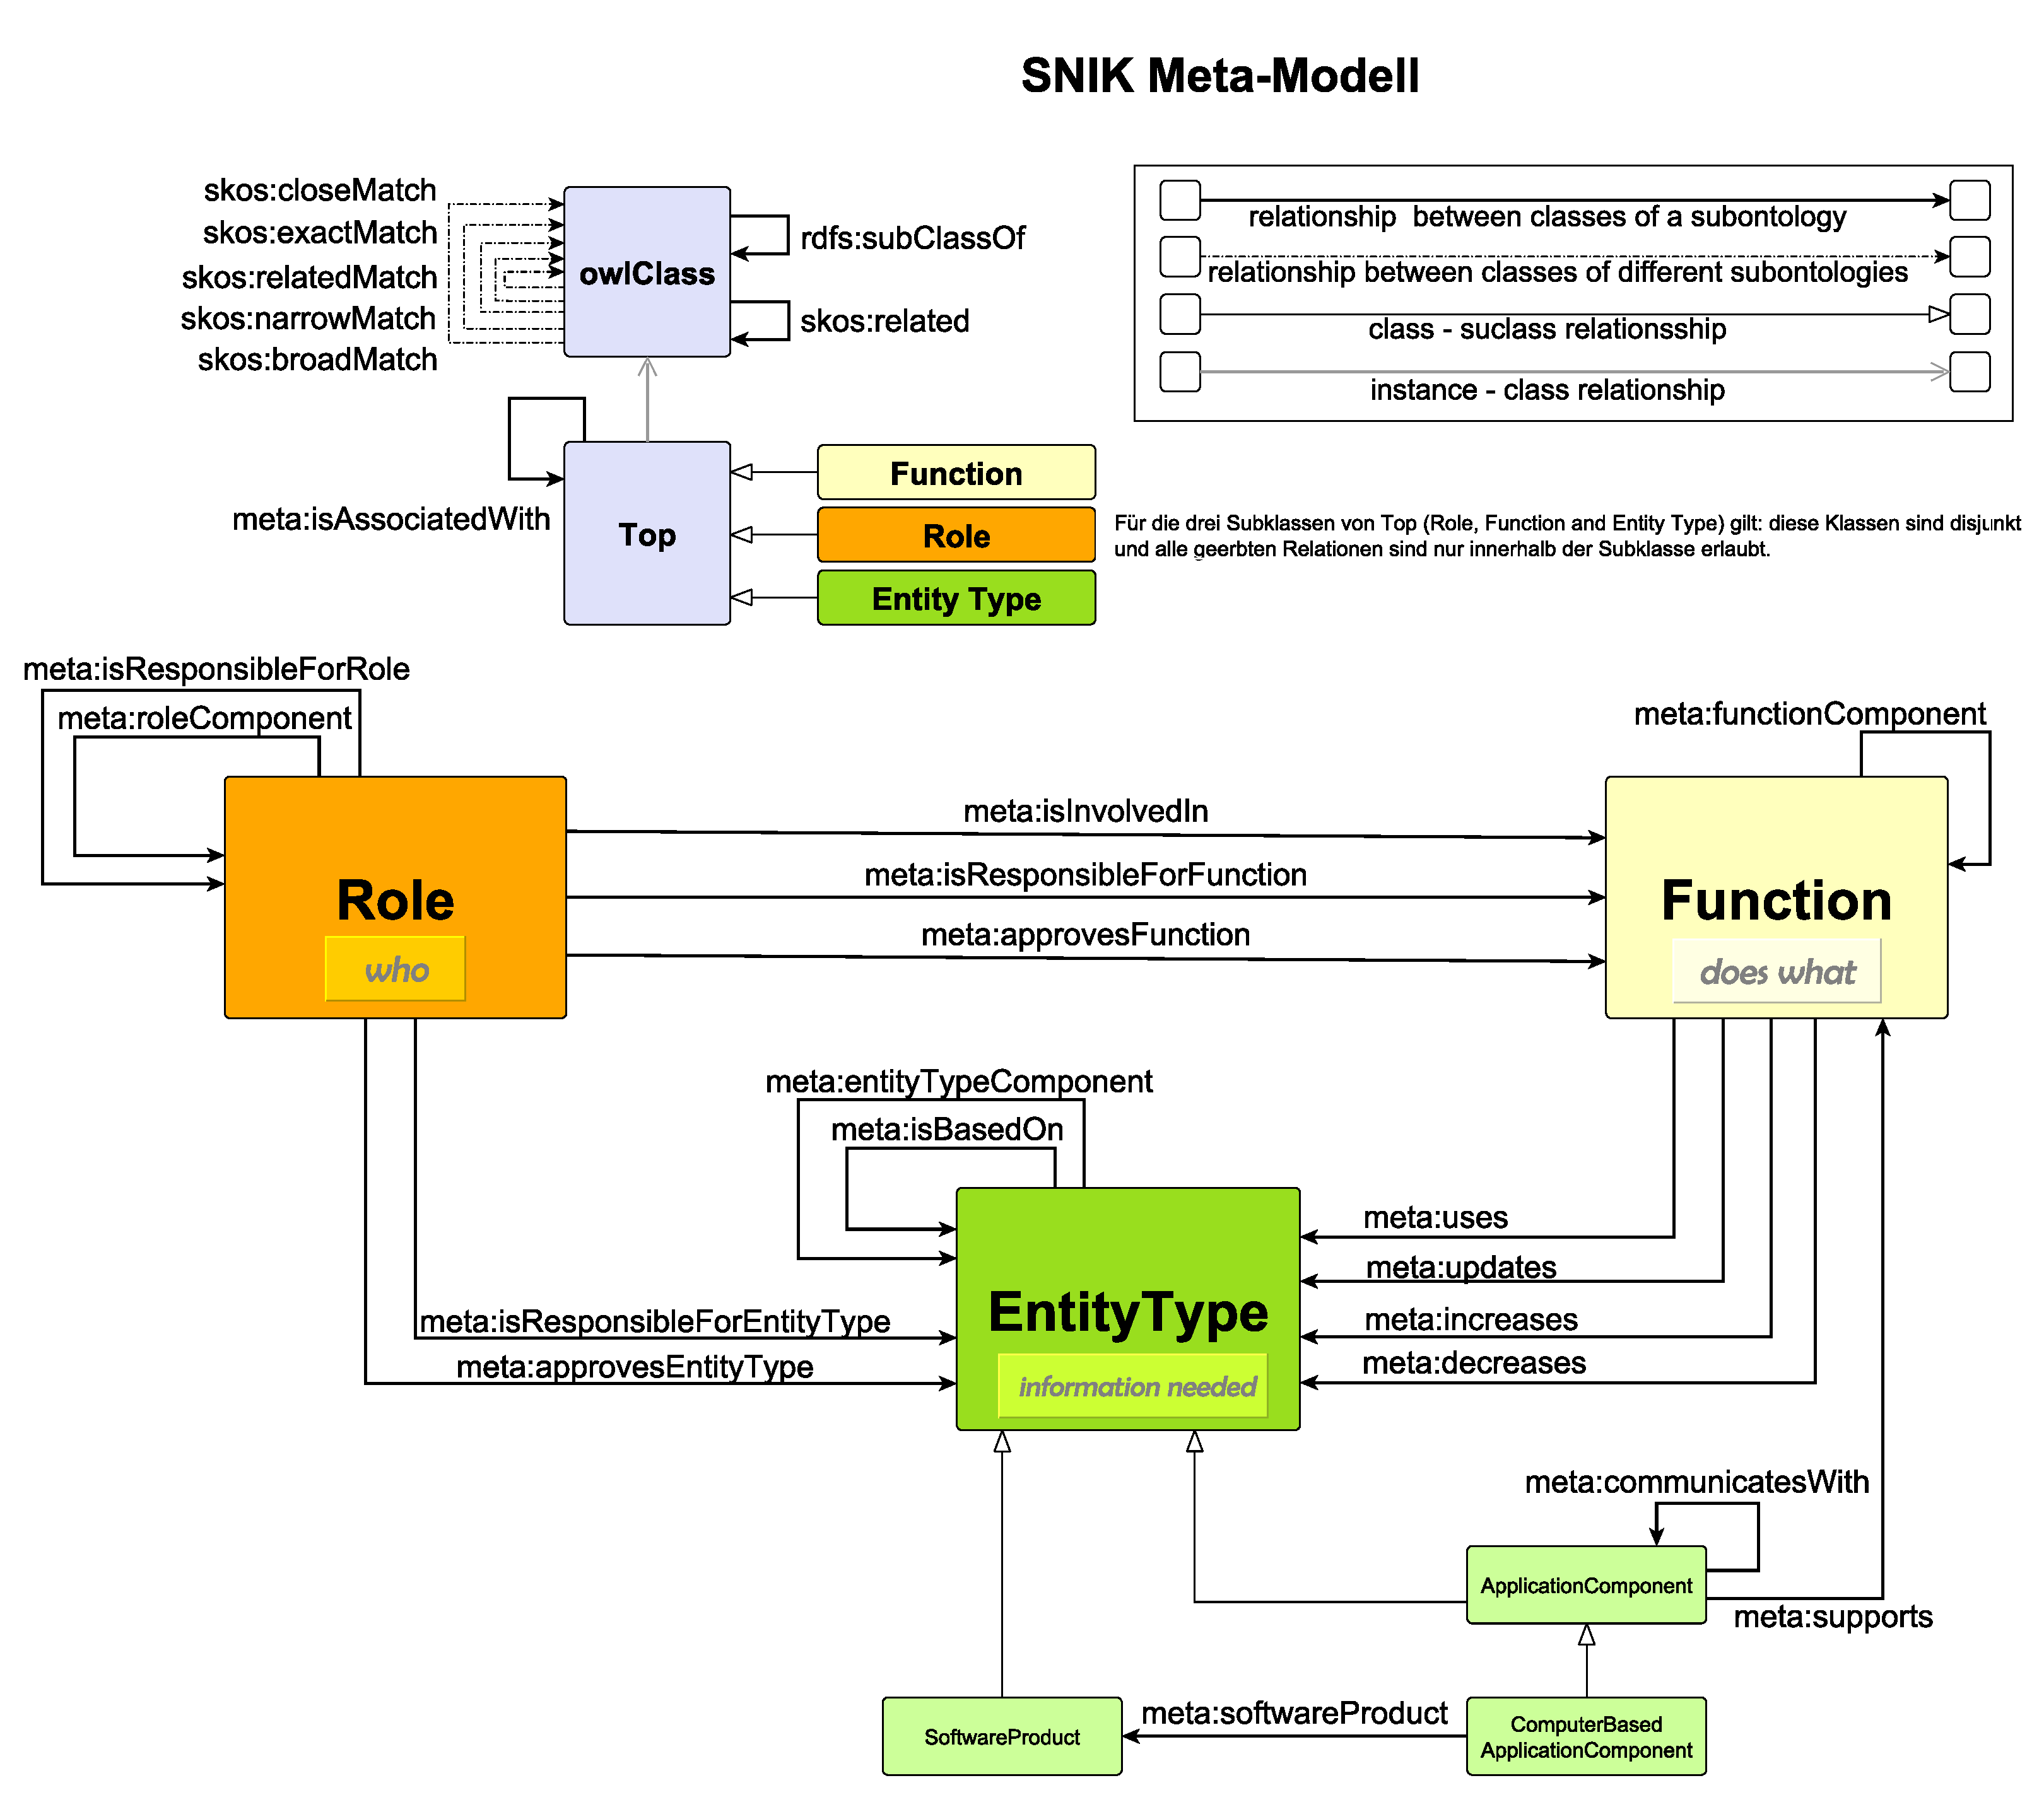
\includegraphics[width=.8\textwidth, height=.9\textheight, keepaspectratio]{Images/snik-metamodel.pdf}
\caption[SNIK Metamodell Version 8]{Das SNIK Metamodell Version 8. Quelle: \url{https://www.snik.eu/public/SNIK_Metamodell_V8.svg}}
\label{fig:snik-metamodel}
\end{sidewaysfigure}

\subsection{\enquote{Eine Ontologie von Ontologien}}

\section{Question Answering-Programme}

Zur Recherche wurden verschiedene Surveys bezüglich \ac{kbqa} bzw. \ac{cdqa} verwendet.
Außerdem wurde über die Herausforderung \ac{qald}, wo mithilfe eines Fragenkatalogs versucht wird, Question Answering-Systeme objektiv zu bewerten.
Als Trainingssatz wird DBpedia verwendet \citep{qald9}.

DBpedia ist eine Ontologie, die aus den Daten Wikipedias besteht.
Es ist das Paradebeispiel für Linked Data und wird häufig zum Training von Question Answering-Programmen genutzt.
Die Daten sind frei und in verschiedenen Formaten, wie z.B. als \ac{rdf}-Tripel, verfügbar.
Über \ac{sparql} können auch direkt online Abfragen getätigt werden.
DBpedia ist außerdem in mehreren Sprachen verfügbar \citep{dbpedia}.

\subsection{gAnswer}

gAnswer wurde von dem Wangxuan Institute of Computer Technology entwickelt und arbeitet mit Wissensbasen, um Question Answering-Aufgaben zu lösen.
Hierfür werden die Fragen in Unterfragen aufgespalten und daraus je ein Syntaxbaum erstellt \citep{ganswer2}.
Es erzielte durch eine durchdachte Vorbereitung der Trainingsdaten sehr schnelle Trainingszeiten bei niedrigem Speicherverbrauch und hoher Genauigkeit bei der Beantwortung von Fragen.
Das Programm hat außerdem die Umformung von natürlicher Sprache in \ac{sparql}-Abfragen als das Problem,
Subontologien zu vergleichen, erkannt, und somit einen neuen Ansatz zur Lösung des Problems der Homonymität geboten.
Das bedeutet, dass Wörter, die verschiedenes bedeuten können, erst nach anfänglicher Lokalisierung des Kontexts betrachtet werden.
Es werden also zuerst Wörter, deren Bedeutung eindeutig ist, betrachtet, und von da aus die kürzeste Verbindung zu einer Bedeutung des fragwürdigen Wortes \citep{ganswerapproach}.
Darauf bauen viele andere Question Answering-Systeme auf.

\subsection{DeepPavlov}
DeepPavlov ist eine open-source Bibliothek zur Entwicklung von Dialogsystemen.
Es ist in \emph{Models} und \emph{Skills} organisiert.
Das System ist hochdynamisch und auf verschiedenste Aufgaben ausgelegt, vor allem aber Dialogsysteme bzw. Chat Bots.
Für Question Answering gibt es bisher nur Ansätze bezüglich \ac{odqa}.

\subsubsection{Architektur}
Ein \emph{Model} ist eine in TensorFlow, eine Schnittstelle für maschinelles Lernen \citep{tensorflow}, implementierte Funktion einer \ac{nlp}-Pipeline,
die sowohl ein neuronales Netz als auch ein nichtneuronales oder regelbasiertes System sein kann.
Models können auch andere Models enthalten.
Ein \emph{Skill} besteht aus Models, jedoch kann er nur Zeichenketten als Ein-/Ausgabe haben.
Sie werden deshalb häufig im Dialog verwendet.
Die Models in Skills werden über einen \emph{Chainer} verbunden, der die Konfigurationsdatei einliest und so die Parameter der Models festsetzt.
Skills und Models werden gleich implementiert und unterscheiden sich nur in den Unterschiedlichen Ein- und Ausgabemöglichkeiten.
Mehrere Skills formen einen \emph{Agent}, wie in \cref{fig:deeppavlov-architektur} sichtbar ist.
Ein Agent kann die verschiedenen Skills, aus denen er besteht, in einer Unterhaltung mit dem Benutzer verwenden und zwischen ihnen wechseln.

\begin{figure}[htbp!]
\centering
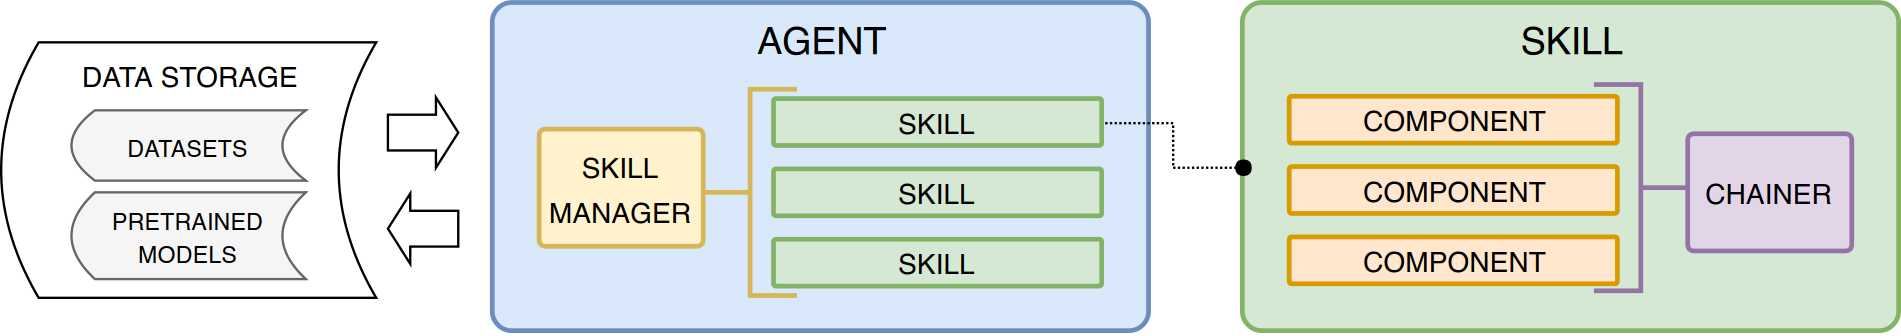
\includegraphics[width=\textwidth, height=\textheight, keepaspectratio]{Images/DeepPavlovArchitecture.png}
\caption[DeepPavlov Architektur]{Die Architektur von DeepPavlov. Quelle: \citet{deeppavlov}}
\label{fig:deeppavlov-architektur}
\end{figure}

\subsection{TeBaQA}

TeBaQA wurde von der DICE group an der Universität Paderborn entwickelt.
Es basiert darauf, 
